\documentclass[a4,10pt]{article} \usepackage[pdftex]{graphicx}
\usepackage{setspace}
\usepackage{hyperref}
\hypersetup{
    colorlinks,%
    citecolor=black,%
    filecolor=black,%
    linkcolor=black,%
    urlcolor=blue
}


\pdfinfo{
   /Author (Ron Keizer, Coen van Hasselt, Pirana Software & Consulting BV)
   /Title  (Pirana Quick Guide)
}

%\usepackage{lineno}
\usepackage{color}
\definecolor{PiranaOrange}{rgb}{0.9,0.4,0.1}
\definecolor{Blue}{rgb}{0.0,0.0,0.7}
\definecolor{Red}{rgb}{0.7,0.0,0.0}
\definecolor{Grey}{rgb}{0.2,0.2,0.2}
\definecolor{grey2}{rgb}{.92, .92, .92}

\bibliographystyle{unsrt}%Choose a bibliograhpic style}
%\usepackage{utopia} %\usepackage{charter} %\usepackage{palatino}
%\usepackage{bookman} %\usepackage{newcent} %\usepackage{times}
%\usepackage[options]{natbib} \sloppy
\renewcommand{\familydefault}{\sfdefault} 
\renewcommand{\emph}[1]{\textbf{\textcolor{Grey}{#1}}} 
\oddsidemargin 1cm
\textwidth 14cm
\textheight 20cm

\begin{document}

{\centering
  \vspace{-100pt}
  \textbf{
    \textcolor{PiranaOrange}{\Large Pirana}
  }\\
  \vspace{5pt} \scriptsize \textcolor{Grey}{The flexible modeling
    environment for NONMEM} \\ \normalsize
  \vspace{12pt}
  \hspace{5pt}
\includegraphics[scale=0.14]{images/pirana_logo.jpg}\\
  \vspace{18pt}
  {\large
    \emph{Quick Guide: Working with, running and manipulating controlstreams in
Pirana}  \vspace{10pt} \\
    Version 1.1
  }

}
\vspace{25pt}


\subsubsection*{Introduction}
\begin{itemize}
\item All models and their associated results available in a folder in
  Pirana are depicted in the main Window.
\item When selecting a model and using the right mouse-button menu, a
  range of actions may be performed on the selected model.
\item Most manipulations (duplicating, removing, etc.) of models are
  available via the sub-menu \emph{Actions} (Figure \ref{fig:Fig1}).
\end{itemize}

%% Fig 1
\begin{figure}[h] \centering
    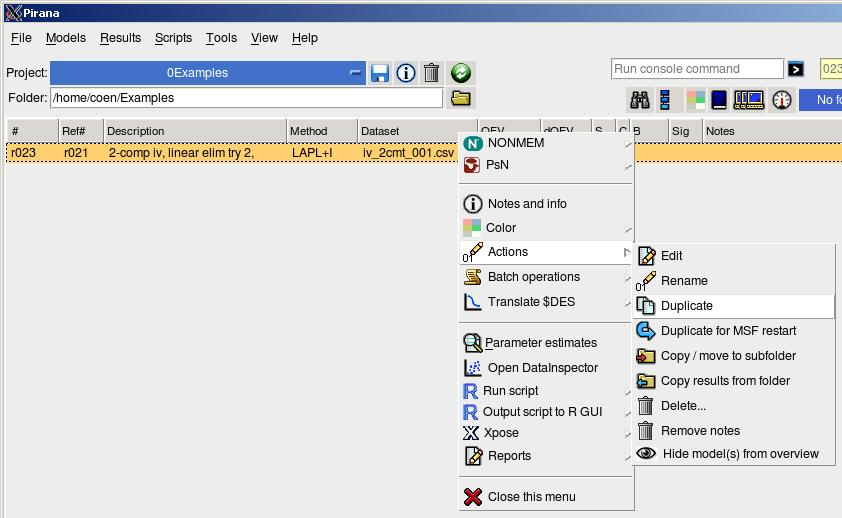
\includegraphics[scale=.4]{images/working_3.jpg}
    \caption{Pirana window with context menu\label{fig:Fig1}}
\end{figure}

%%%%%%%%%%%%%%%%%%%

\subsubsection*{Running a model}
\begin{itemize}
\item Select the model and open the right-mouse button context menu.
\item Select the preferred methode of running the model, i.e. NONMEM $
  \rightarrow$ nmfe, or PsN $ \rightarrow$ execute. 
\item If you are using nmfe to run a model, NONMEM has to be
  registered within Pirana first (refer to the Quick Guide on
  installing NONMEM). If PsN is installed, Pirana will automatically
  recognize this.
\end{itemize}

%%%%%%%%%%%%%%%%%%%

\subsubsection*{Running a model using nmfe} 
After having selected Run via nmfe, the Run window depicted in Figure
\ref{fig:Fig2} will appear. A number of options are available here, before
executing the run.
\begin{itemize}
\item \emph{NONMEM}: The preferred NONMEM installations may be selected. 
\item \emph{Run in seperate folder(s)}: A NONMEM run may be executing
  in a sub-folder, to enable to run multiple runs
  simultaneously. Results from a subfolder can be imported to the main
  folder in Pirana.
\item \emph{Run in background}: No console window is opened, the model
  is run in the background.
\item \emph{Clusters-Submit to SGE}: Run on a cluster using SGE (optional). 
\item \emph{Clusters-Parallelization}: Run using parallelization
  available in NONMEM 7.2 (optional).
\item \emph{Connect to}: Cluster (optional). Connect to a
  cluster. Please refer to the Quick Guide on Clusters for more information.
\item \emph{Script contents}: The script which is executed to run the model.
\item The run may be executed using the \emph{\Large{$>$}} button.
\end{itemize}

%% Fig 2
\begin{figure}[h] \centering
    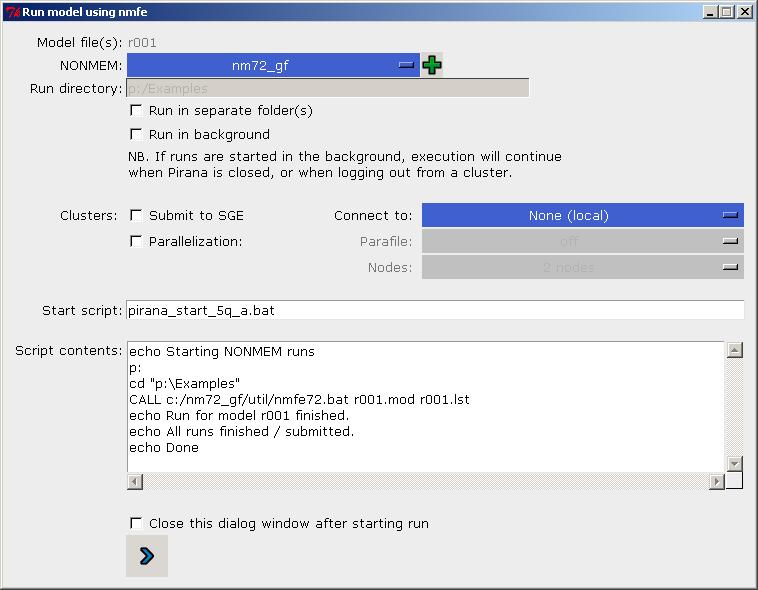
\includegraphics[scale=.4]{images/working_4.jpg}
    \caption{Run window for nmfe\label{fig:Fig2}}
\end{figure}

%%%%%%%%%%%%%%%%%%%

\subsubsection*{Running a model using PsN} 
After having selected Run via PsN, the PsN run window depicted in
Figure \ref{fig:Fig3} will appear. Again, a number of options are available here,
before executing the run.
\begin{itemize}
\item \emph{Cluster}: Cluster to connect to (optional). Please refer
  to the Quick Guide on Clusters for more information.
\item \emph{NONMEM}: The preferred NONMEM installations may be
  selected. 
\item \emph{Run in background}: After executing the model, output is
  not printed to the screen.
\item \emph{PsN command line}: This is the command line which is
  executed. Additional PsN arguments may be added here.
\item The top part of the window shows an overview for of available
  PsN arguments.
\end{itemize}

%% Fig 3
\begin{figure}[h] \centering
    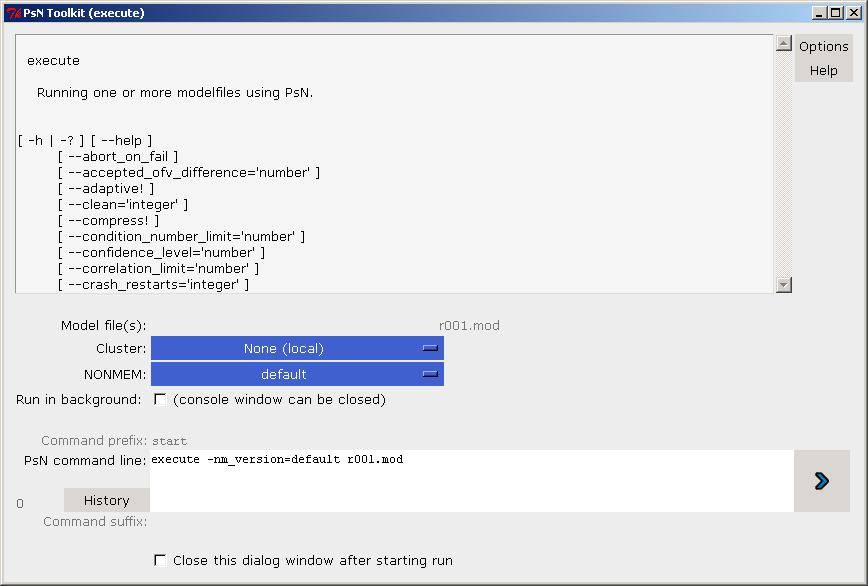
\includegraphics[scale=.4]{images/working_5.jpg}
    \caption{Run window for PsN\label{fig:Fig3}}
\end{figure}

%%%%%%%%%%%%%%%%%%%

\subsubsection*{Generating an empty control stream}
\begin{itemize}
\item An empty control stream may be generated via  Models $ \rightarrow$  New model (Figure \ref{fig:Fig4}).
\item Choose the template control stream that you want to use.
\item The control stream will be opened in the text editor defined in Settings.
\end{itemize}

%% Fig 4
\begin{figure}[h] \centering
    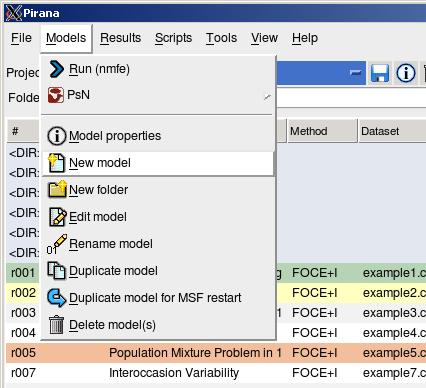
\includegraphics[scale=.5]{images/working_1.jpg}
    \caption{Create an empty model\label{fig:Fig4}}
\end{figure}

\subsubsection*{Generating a new control stream using the Wizard}
\begin{itemize}
\item Empty, partly pre-coded PK models may be generated using the Wizard (Tools $ \rightarrow$ Wizards). 
\item In the Wizards menu (Figure \ref{fig:Fig5}), select PK NONMEM model. 
\item After finishing the Wizard, a new control stream will be created and opened in the editor.
\end{itemize}

%% Fig 5
\begin{figure}[h] \centering
    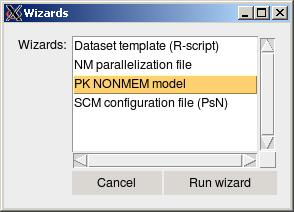
\includegraphics[scale=.5]{images/working_2.jpg}
    \caption{Create a new model using the Wizard\label{fig:Fig5}}
\end{figure}

\subsubsection*{Editing  a control stream}
\begin{itemize}
\item A control stream visible in the main Pirana window may be edited by double clicking on the model.
\item Alternatively, this may be done through the right-mouse button menu Actions $ \rightarrow$ Edit.
\item Please note that an alternative code editor can be defined
  through File $ \rightarrow$ Settings $ \rightarrow$ Software
  integration. The default in Pirana is notepad.exe, but it is highly
  recommended to change this to an appropriate code editor such as
  Emacs, ConText, or PSPad.
\end{itemize}

\subsubsection*{Duplicating a control stream}
\begin{itemize}
\item A control stream may be duplicated through the right-mouse
  button menu Actions $ \rightarrow$ Duplicate (Figure \ref{fig:Fig1}).
\item In the resulting Duplication window (Figure \ref{fig:Fig6}), you can choose
  to update parameter estimates in the new file to the ones estimated
  for the current model, fix the parameter estimates, change the
  file numbers in \$TABLE and \$EST records.
\item Please note that to correctly duplicate with updated parameter
  estimates, you are required to adhere to some coding guidelines,
  especially for the \$OMEGA and \$SIGMA blocks. See the Pirana manual
  for more information.
\item After pressing the Duplicate button, a new model will be created
  and opened in the editor.
\end{itemize}

%% Fig 6
\begin{figure}[h] \centering
    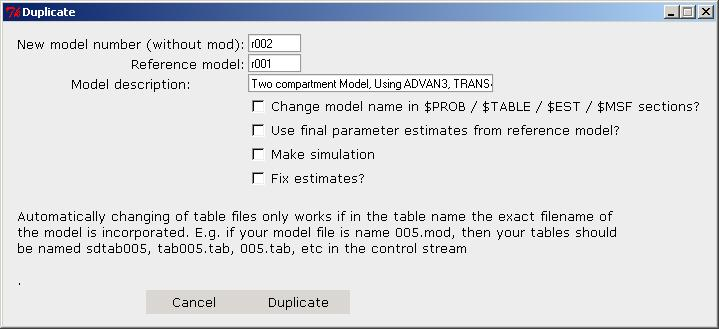
\includegraphics[scale=.5]{images/working_6.jpg}
    \caption{Create a new model using the Wizard\label{fig:Fig6}}
\end{figure}

\subsubsection*{Renaming a control stream}
\begin{itemize}
\item A control stream may be renamed through the right-mouse
  button menu Actions $\rightarrow$ Rename (Figure \ref{fig:Fig1}). Some of the
  same options as under duplication are available.
\end{itemize}

\subsubsection*{Deleting a control stream}
\begin{itemize}
\item A control stream may be deleted by selecting the right-mouse
  button menu Actions $\rightarrow$ Delete (Figure \ref{fig:Fig1}). Alternatively,
  a can be selected and subsequently the keyboard button DELETE can be
  pressed.
\item In the dialog that is opened, you can select what to delete:
  only the control stream (models), or also the associated results
  files, datasets. If you have selected one or more folders in the
  main overview to be deleted, the 'folder' option should be checked to
  actually delete these as well.
\end{itemize}

\subsubsection*{Viewing parameter estimates inside the GUI}

\begin{itemize}
\item During model building, parameter estimates can be viewed by selecting a run, and opening the Estimates Tab on the right panel (Figure \ref{fig:Fig7}).
\item The parameter estimates window can be opened from the option Parameter estimates in the context menu (right mouse button) (Figure \ref{fig:Fig8}), or alternatively from the button in the right panel with estimates. 
\item Results from the table can be exported to CSV, LaTeX or HTML, and different transformations of variances can be selected.
\item When selecting multiple runs, parameter estimates can be compared with each other (Figure \ref{fig:Fig9}). 
\end{itemize}

\begin{figure}[h] \centering
    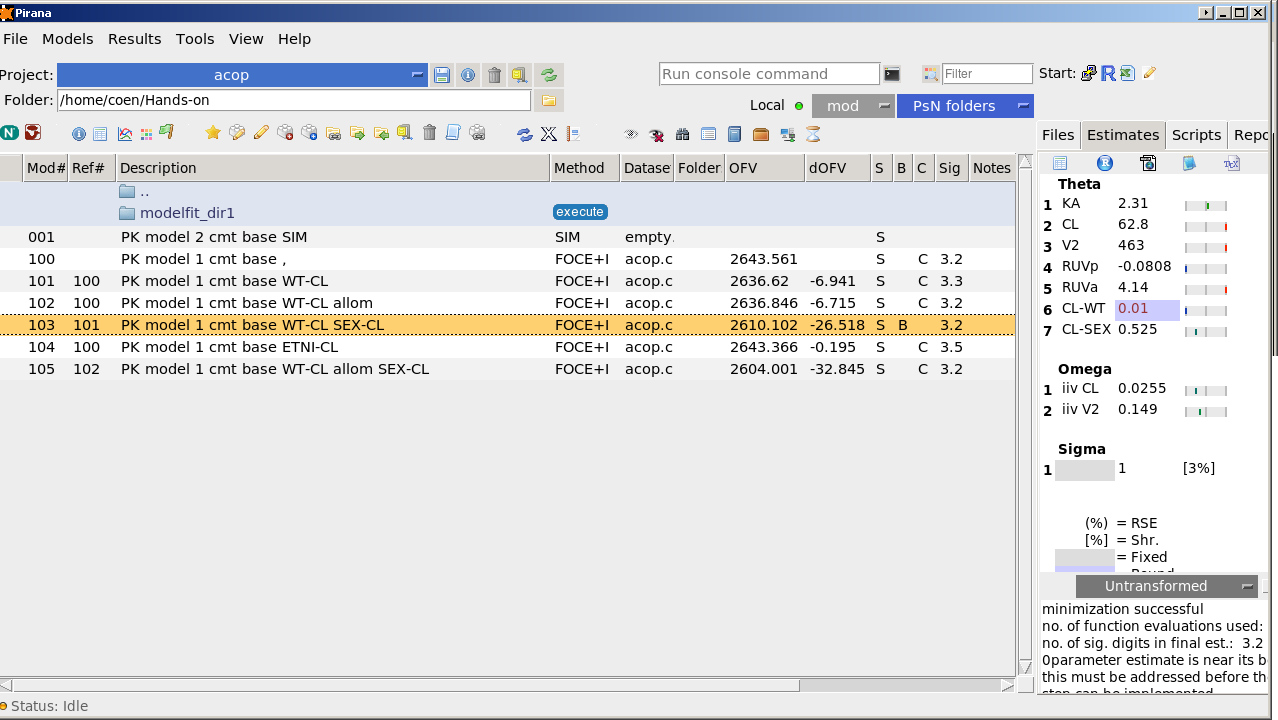
\includegraphics[scale=.25]{images/report_1.png}
    \caption{Viewing estimates in right panel in the Pirana GUI\label{fig:Fig7}}
\end{figure}

\begin{figure}[h] \centering
    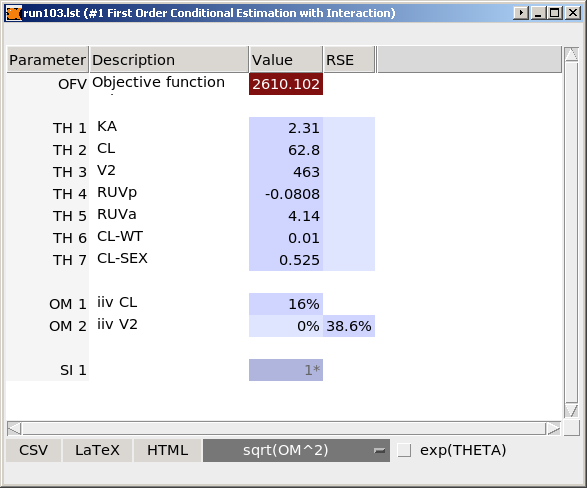
\includegraphics[scale=.35]{images/report_2.png}
    \caption{Parameter estimates window\label{fig:Fig8}}
\end{figure}

\begin{figure}[h] \centering
    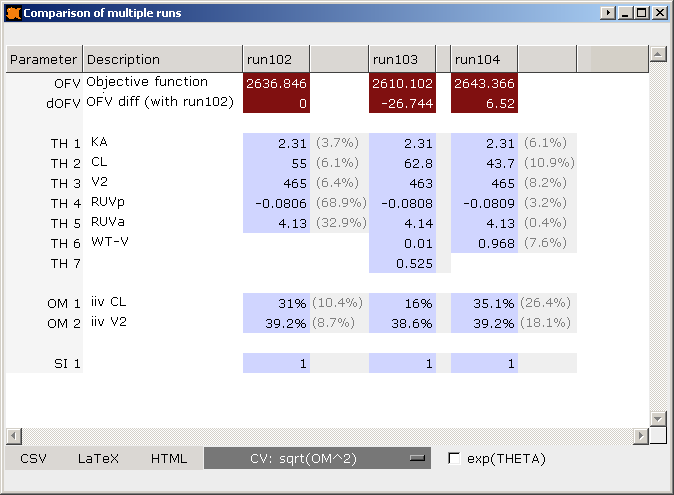
\includegraphics[scale=.35]{images/report_4.png}
    \caption{Parameter estimates comparison\label{fig:Fig9}}
\end{figure}



\end{document}
